% !TEX encoding = UTF-8 Unicode
% !TEX root =  ../Bachelorarbeit.tex

\chapter{\"Uberblick}
\label{UeberblickEntwicklungsplattform}

Die Auswahl einer geeigneten Entwicklungsplattform bildet die Grundlage f\"ur die erfolgreiche Implementierung und Evaluierung eingebetteter Systeme. Im Rahmen dieser Arbeit dient der MSP430FR5729 von Texas Instruments als zentrale Hardwarekomponente. Dessen Architektur und Funktionalit\"aten werden in den folgenden Abschnitten n\"aher betrachtet.

Der MSP430FR5729 ist ein Low-Power-Microcontroller  \Fachbegriff[Mikrocontroller mit 16-Bit-Registerbreite und reduzierter Befehlssatzarchitektur (Reduced Instruction Set Computer)]{16-Bit-RISC-Microcontroller} von Texas Instruments mit einer Maximalen Taktfrequenz von Acht \Fachbegriff[Ma{\ss}einheit für die Frequenz und entspricht einer Million Schwingungen pro Sekunde (1 MHz = 10$^{6}$ Rechenschritte).]{Megaherz}. Eingebaute Low-Power-Modi (\Abkuerzung{Low Power Mod}{LPM}s), (Auflistung aller Modi in \Abbildung{operation_modes}) erm\"oglichen \ua niedrigere Taktfrequenzen und das deaktivieren von Oszillatoren, wodurch er sich besonders gut f\"ur energieeffiziente Anwendungen im Bereich eingebetteter Systeme eignet. \Zitat[S. 43, Kap. 6.3, S. 35, Kap. 1.4 \& S. 37, Kp. 1.4.1]{ti:slase35c, ti:slau272d}

\begin{figure}[h!]
	\centering
	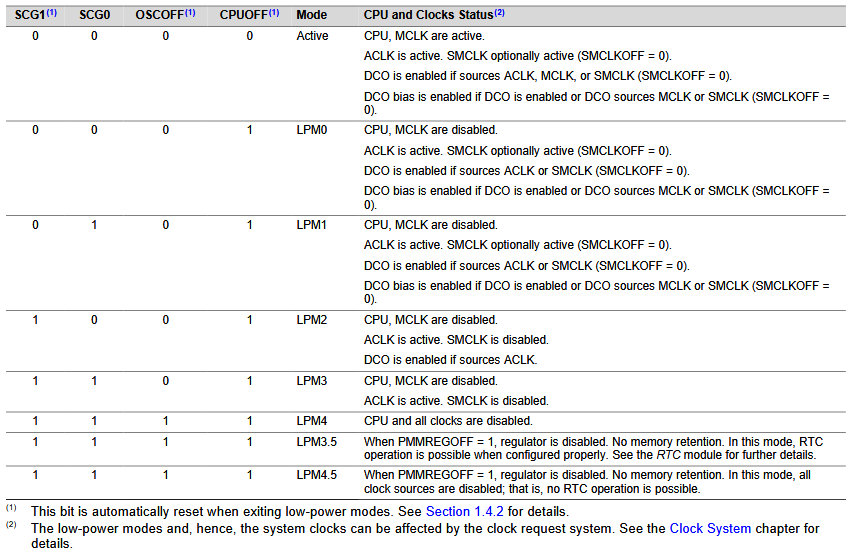
\includegraphics[width=1.0\textwidth]{../Bilder/Operating_Modes.png}
	\caption{Operating Modes\\\Zitat[S. 37, Kap. 1.4, Tab. 1-2]{ti:slau272d}}
	\label{fig:operation_modes}
\end{figure}

Der Mikroprozessor besitzt 16 Kilobyte an nicht-fl\"uchtigen FRAM, sowie ein Kilobyte \Fachbegriff[Schnellster, fl\"uchtiger Speicher mit geringer Kapazit\"at, bestehend aus Flip-Flops welcher meist direkt in der CPU mit eingebaut ist.]{statischen Arbeitsspeicher} (\Abkuerzung{Static Random Access Memory}{SRAM}). 

Die Versorgungsspannung betr\"agt 2 bis 3,6 Volt wobei ebenfalls verschiedene Low-Power-Modi verwendet werden k\"onnen, um den Stromverbrauch zunehmend zu minimieren. Diese beeinflussen den sp\"ateren Umgang mit Timer-Interrupts, weil sie den Energieverbrauch im Wartezustand beeinflussen. \Zitat[S. 26, Kap. 5.20]{ti:slase35c}

Des Weiteren besitzt der Chip F\"unf Interne 16-Bit Timer mit jeweils Sieben\\\NeuerBegriff{Capture and Compare} Registerbl\"ocken. Diese internen Timer stellen eine zentrale Komponente f\"ur die Realisierung pr\"aziser Zeitgesteuerter Funktionen und die Generierung von Interrupts dar, welche im nachfolgenden Kapitel \ref{TIMER&ISR} tiefgreifender erl\"autert werden.

Zur externen Kommunikation sind Protokolle wie \Abkuerzung{Universal Asynchronous Receiver Transmitter}{UART}, \Abkuerzung{Inter-Integrated Circuit}{I$^{2}$C} und \Abkuerzung{Serial Peripheral Interface}{SPI} integriert, welche mit 32 Programmierbaren \Abkuerzung{General Purpose Input/Output}{GPIO}-Pins angeschlossen werden k\"onnen. Kommunikationsschnittstellen sind f\"ur die Interaktion mit der Au{\ss}enwelt und Peripherieger\"aten von hoher Bedeutung. Eine detailliertere Ausarbeitung des \Fachbegriff[Serielle Schnittstelle in Mikrocontrollern von Texas Instruments, die verschiedene Kommunikationsprotokolle (\zB UART, SPI, I$^{2}$C) unterst\"utzt.]{enhanced Universal Serial Communication Interface} (\Abkuerzung{enhanced Universal Serial Communication Interface}{eUSCI}) in Kapitel \ref{eUSCI}. \Zitat[S. 1, Kap. 1.1]{ti:slase35c}

\begin{figure}[h!]
	\centering
	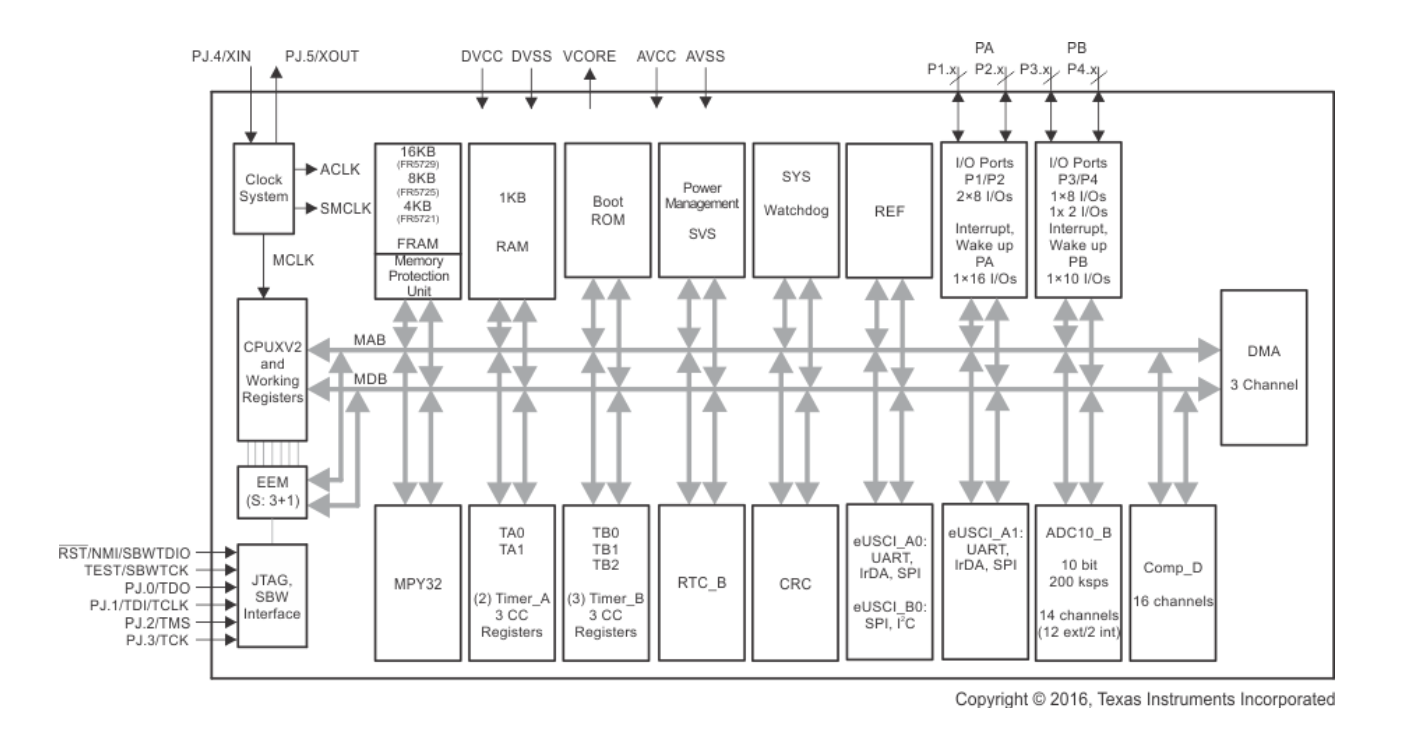
\includegraphics[width=1.0\textwidth]{../Bilder/FunctionalBlockDiagram_MSP430FR5729.png}
	\caption{Block Diagramm MSP430FR5729\\Mikrocontroller \Zitat[S. 2, Kap. 1.4]{ti:slase35c}}
	\label{fig:BlockDiagramm_msp430}
\end{figure}

\newpage
\Abbildung{BlockDiagramm_msp430} zeigt ein vollst\"andiges Block Diagramm des Mikroprozessors, welches noch einige weitere Eigenschaften, Funktionen und Subsysteme auflistet. \AI


\section{Timer und Interrupt Service Routinen (ISR)}
\label{TIMER&ISR}

Timer und Interrupt Service Routinen (\Abkuerzung{Interrupt Service Routine}{ISR}s) stellen einen fundamentalen Baustein moderner eingebetteter Systeme dar. Sie erm\"oglichen pr\"azise, zeitgesteuerte Funktionen als auch das reagieren auf externe Ereignisse. Womit die Realisierungen komplexer, Echtzeitsysteme m\"oglich wird. Im Folgenden wird die Timer-Architektur des MSP430FR5729 und die zugeh\"origen ISR-Mechanismen detailliert betrachtet.

Der MSP430FR5729 verf\"ugt \"uber insgesamt f\"unf 16-Bit-Timer, wobei zwei dem Typ A und drei dem Typ B angeh\"oren. Beide Typen erm\"oglichen vielseitige Zeitsteuerungsfunktionen, weisen jedoch spezifische Unterschiede in ihren Konfigurationsm\"oglichkeiten auf.

Beide Timer-Typen verf\"ugen \"uber einen gemeinsamen 16-Bit-Z\"ahler sowie sieben Capture/Compare-Register. Diese Register erm\"oglichen die Implementierung verschiedenster Funktionen. Die Capture-Funktionalit\"at dient dazu, den aktuellen Z\"ahlerwert bei einem externen oder internen Ereignis pr\"azise zu erfassen. Dies ist beispielsweise n\"utzlich f\"ur die Messung von Pulsweiten oder Frequenzen. Die Compare-Funktionalit\"at hingegen erlaubt den Vergleich des aktuellen Z\"ahlerstandes mit einem in den Compare-Registern hinterlegten Wert. Bei einer \"ubereinstimmung kann eine konfigurierbare Aktion ausgel\"ost werden, wie beispielsweise das Setzen oder R\"ucksetzen eines Ausgangspins oder das Generieren eines Interrupts. Die vielseitigen Einstellungsm\"oglichkeiten dieser Register erlauben die Realisierung komplexer Zeitgesteuerter Aufgaben. \Zitat[S. 333, Kap. 11 \& S. 355, Kap. 12, S. 287, Kap. 8.3 \& S. 194, Kap. 6.8.2]{ti:slau272d,davies:msp430}

Die Timer des Typs B weisen im Vergleich zu dem Timer des Typs A, erweiterte Konfigurationsm\"oglichkeiten auf. Darunter fällt die Konfigurierbarkeit der Timer-L\"ange auf 8, 10, 12 oder 16 Bit, was eine flexible Anpassung der Z\"ahlaufl\"osung und der \"uberlaufperiode f\"ur unterschiedliche Aufl\"osungen erm\"oglicht. Weiterhin sind alle Capture/Compare-Bl\"ocke doppelt gepuffert. Diese doppelte Pufferung erlaubt das Laden neuer Vergleichswerte, w\"ahrend eines aktiven Z\"ahlzyklus, wodurch unerw\"unschte Effekte oder Inkonsistenzen in den Ausgangssignalen vermieden werden. Zudem k\"onnen alle Ausg\"ange auf einen hochohmigen Zustand umgeschaltet werden, was in bestimmten Applikationen vorteilhaft sein kann. Ein weiterer wichtiger Unterschied besteht darin, dass die Capture/Compare-Eing\"ange nicht synchronisiert sind und somit asynchron zu dem internen Takt des Timers operieren k\"onnen, was in bestimmten Szenarien die Erfassung externer Ereignisse erleichtert. \Zitat[S. 356, Kap. 12.1.1, S. 353, Kap. 8.9]{ti:slau272d, davies:msp430}

F\"ur die pr\"azise Steuerung und Ereignisbehandlung bieten die Timer verschiedene Betriebsarten, die im Folgenden n\"aher erl\"autert werden.

\newpage
\subsection{Timer Zählweisen}
\label{Timer_CountMode}

Der Z\"ahlmodus, bestimmt die interne Z\"ahlweise des Timers. Die Timer unterst\"utzen typischerweise mehrere Varianten dieses Modus, um unterschiedlichen Anforderungen gerecht zu werden. \Zitat[S. 291, Kap. 8.3.1]{davies:msp430}

\begin{itemize}
	\item \textbf{Up Mode:} Im Up Mode (Additive Z\"ahlweise) beginnt der Z\"ahler bei Null und inkrementiert seinen Wert mit jedem Taktimpuls der gew\"ahlten \Fachbegriff[Eine Referenz auf ein periodisches Zeitsignal um zeitliche Abl\"aufe zu synchronisieren; typischerweise in Form von Quarzoszillatoren oder externen Taktsignalen.]{Clock-Source}. Er erreicht einen vordefinierten Maximalwert, der im Compare-Register gespeichert ist, und beginnt dann wieder von Null zu z\"ahlen. Ein \"uberlauf-Interrupt wird generiert, sobald der Z\"ahler den Wert von CCR0 erreicht. Dieser Modus eignet sich ideal f\"ur die Erzeugung periodischer Ereignisse oder die Messung von Zeitintervallen bis zu einem bestimmten Grenzwert. Beispielsweise kann durch die Wahl einer geeigneten Clock-Source und eines passenden Wertes im Compare-Register eine pr\"azise Zeitbasis f\"ur periodische Aufgaben geschaffen werden. \Zitat[S. 337, Kap. 11.2.3.1 \& S. 359, Kap. 12.2.3.1, S. 330, Kap. 8.6]{ti:slau272d, davies:msp430}
	
	\item \textbf{Continuous Mode:} Der Continuous Mode l\"asst den Z\"ahler von Null bis zum maximal m\"oglichen Wert (FFFFh f\"ur 16-Bit-Timer) z\"ahlen und anschlie{\ss}end wieder bei Null beginnen. Ein \"uberlauf-Interrupt wird generiert, wenn der Z\"ahler vom Wert von FFFFh auf 0 \"uberl\"auft. \Zitat[S. 338, Kap. 11.2.3.2 \& S. 360, Kap. 12.2.3.2]{ti:slau272d} Dieser Modus ist besonders n\"utzlich, wenn l\"angere, voneinander unabh\"angige Zeitintervalle zu messen oder wenn eine freilaufende Zeitbasis ben\"otigt wird, um Ereignisse in Bezug auf den Z\"ahlerstand, ohne einen periodischen Neustart durch das Compare-Register, zu erfassen. \Zitat[S. 338, Kap. 11.2.3.3 \& S. 360, Kap. 12.2.3.3, S. 318, Kap. 8.5]{ti:slau272d, davies:msp430}

	\item \textbf{Up/Down Mode:} Der Up/Down Mode (Auf-/Abw\"artsz\"ahlmodus) kombiniert das Auf- und Abz\"ahlen. Der Z\"ahler beginnt bei Null, z\"ahlt Zyklisch bis zum festgelegten Wert im Compare-Register und dann wieder bis Null herunter. Ein \"uberlauf-Interrupt wird generiert, wenn der Z\"ahler den Wert von CCR0 erreicht, und ein weiterer Interrupt (sofern aktiviert) kann beim Erreichen von Null gesetzt werden. \Zitat[S. 339, Kap. 11.2.3.4 \& S. 361, Kap. 12.2.3.4]{ti:slau272d} Dieser Modus erzeugt eine symmetrische \Fachbegriff[Ein Verfahren zur Steuerung der Leistungszufuhr, bei dem die mittlere Ausgangsleistung durch Variieren des Abtastverh\"altnisses eines Rechtecksignals reguliert wird.]{Pulsweitenmodulation (PWM)} und wird h\"aufig in Anwendungen zur Motorsteuerung oder zur Erzeugung pr\"aziser analoger Ausgangssignale eingesetzt. \Zitat[S. 340, Kap. 11.2.3.5 \& S. 362, Kap. 12.2.3.5, S. 349, Kap. 8.7]{ti:slau272d, davies:msp430}
\end{itemize}

Die Wahl eines geeigneten Modus h\"angt stark von der spezifischen Anwendung ab. F\"ur einfache Zeitmessungen oder periodische Aufgaben ist der Up Mode oft ausreichend, w\"ahrend der Continuous Mode f\"ur l\"angere Intervalle oder als Basis f\"ur komplexere Zeitsteuerungen dient. Der Up/Down Mode hingegen findet seine Anwendung prim\"ar in der Erzeugung von Steuersignalen.

\subsection{Capture-Mode}
\label{Timer_CaptureMode}

Der Capture Mode erm\"oglicht es, den aktuellen Wert des Z\"ahlers pr\"azise zu erfassen, wenn ein bestimmtes Ereignis an einem zugeh\"origen Eingangspin auftritt. Der erfasste Z\"ahlerwert wird in einem der Capture-Register (CCR0 bis CCR6) gespeichert. Dies ist besonders n\"utzlich f\"ur die Messung von externen Signalen wie Pulsweiten, Frequenzen oder der Zeit zwischen zwei Ereignissen. Beispiele hierzu in \Abbildung{CaptureModeBeispiele}.

\begin{figure}[h!]
	\centering
	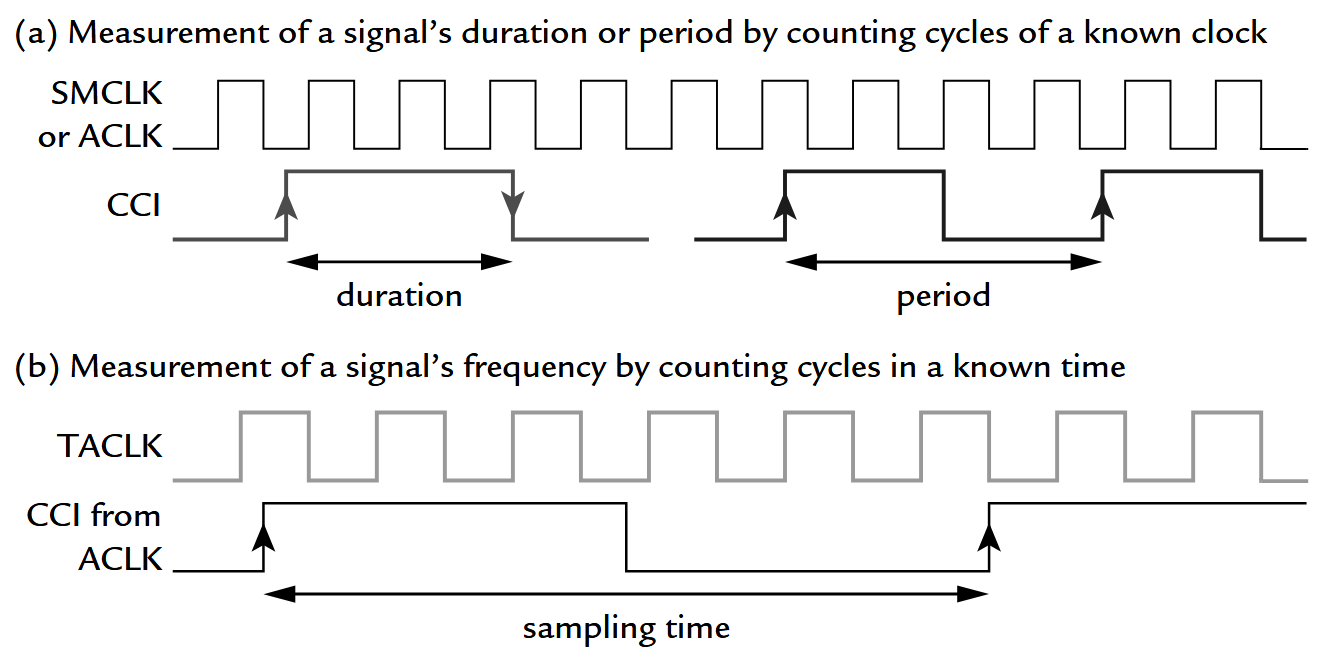
\includegraphics[width=1.0\textwidth]{../Bilder/CaptureMode_Beispiele.png}
	\caption{Capture Mode Einsatzbeispiele\\\Zitat[S. 301, Abb. 8.7]{davies:msp430}}
	\label{fig:CaptureModeBeispiele}
\end{figure}

Die Timer des MSP430FR5729 unterst\"utzen verschiedene Capture-Modi. Diese legen fest, bei welcher Art von Signal\"anderung die Erfassung des Z\"ahlerwertes erfolgt:

\begin{itemize}
	\item \textbf{Capture on rising edge:} Sobald am zugeh\"origen Eingangspin eine steigende Flanke detektiert wird (\"ubergang von Low nach High) wird in diesem Modus der aktuelle Z\"ahlerwert in das Capture-Register geschrieben.

	\item \textbf{Capture on falling edge:} Hier erfolgt die Erfassung des Z\"ahlerwertes am Eingangspin bei einer fallenden Flanke (\"ubergang von High nach Low).

	\item \textbf{Capture on both edges:} Dieser Modus erm\"oglicht die Erfassung des Z\"ahlerwertes sowohl bei steigender als auch fallender Flanken. Dies ist besonders praktisch f\"ur die Messung von Signalperioden oder bei Relevanz beider Flanken eines Signals.
\end{itemize}

Sofern ein Interrupt im entsprechenden Capture-Register aktiviert ist, kann dieser auch Interrupts ausl\"osen. In der zugeh\"origen ISR kann der erfasste Z\"ahlerwert aus dem Capture-Register gelesen und weiterverarbeitet werden. Mehrere Capture-Register innerhalb eines Timers erm\"oglichen die Erfassung und Auswertung mehrerer aufeinanderfolgender Ereignisse, ohne dass der vorherige Wert \"uberschrieben wird. 

Die Konfiguration des Capture Mode umfasst die Auswahl des ausl\"osenden Ereignisses (Flanke) sowie \ggf die Aktivierung des Capture-Interrupts. Die erfassten Zeitstempel im Capture-Register erlauben pr\"azise Messungen und die Analyse externer Signale in eingebetteten Systemen. \Zitat[S. 340, Kap. 11.2.4.1 \& S. 362, Kap. 12.2.4.1, S. 300, Kap. 8.4]{ti:slau272d, davies:msp430}

\subsection{Compare-Mode}
\label{Timer_CompareMode}

Der Compare Mode erm\"oglicht es, den aktuellen Wert des Z\"ahlers kontinuierlich mit den in den Compare-Registern CCR0 bis CCR7 hinterlegten Werten zu vergleichen. Wenn der Z\"ahlerstand mit dem Vergleichswert \"ubereinstimmt, kann \zB ein Interrupt ausgel\"ost oder ein Ausgangspin beeinflusst werden.

Die Compare-Modi bieten verschiedene M\"oglichkeiten, wie der Ausgangspin bei einer \"ubereinstimmung beeinflusst werden soll:

\begin{itemize}
	\item \textbf{Set output on compare:} Bei einer \"ubereinstimmung des Z\"ahlerstandes mit dem Compare-Registerwert wird der zugeh\"orige Ausgangspin auf High gesetzt.

	\item \textbf{Reset output on compare:} Hier wird der Ausgangspin bei \"ubereinstimmung auf Low gesetzt.

	\item \textbf{Toggle output on compare:} In diesem Modus \"andert der Ausgangspin bei jeder \"ubereinstimmung seinen Zustand (von High nach Low oder von Low nach High).

	\item \textbf{Output High:} Der Ausgangspin wird permanent auf High gehalten.

	\item \textbf{Output Low:} Der Ausgangspin wird permanent auf Low gehalten.

	\item \textbf{Set/Reset:} In Kombination mit dem Compare-Register 0 (CCR0) kann ein PWM-Signal erzeugt werden. Beispielsweise kann der Ausgang bei Erreichen des CCR0-Wertes gesetzt und bei Erreichen des CCRn-Wertes zur\"uckgesetzt werden (oder umgekehrt), wobei CCRn die Pulsweite bestimmt.
\end{itemize}

\Abbildung{OutputUnit_UpDown_Mode} zeigt eine m\"ogliche Konfiguration im Z\"ahlmodus Up/Down mit zwei Compare-Registern (TAxCCR1 \& TAxCCR2), eingestellt auf Toggle/Set und Toggle/Reset.

\begin{figure}[h!]
	\centering
	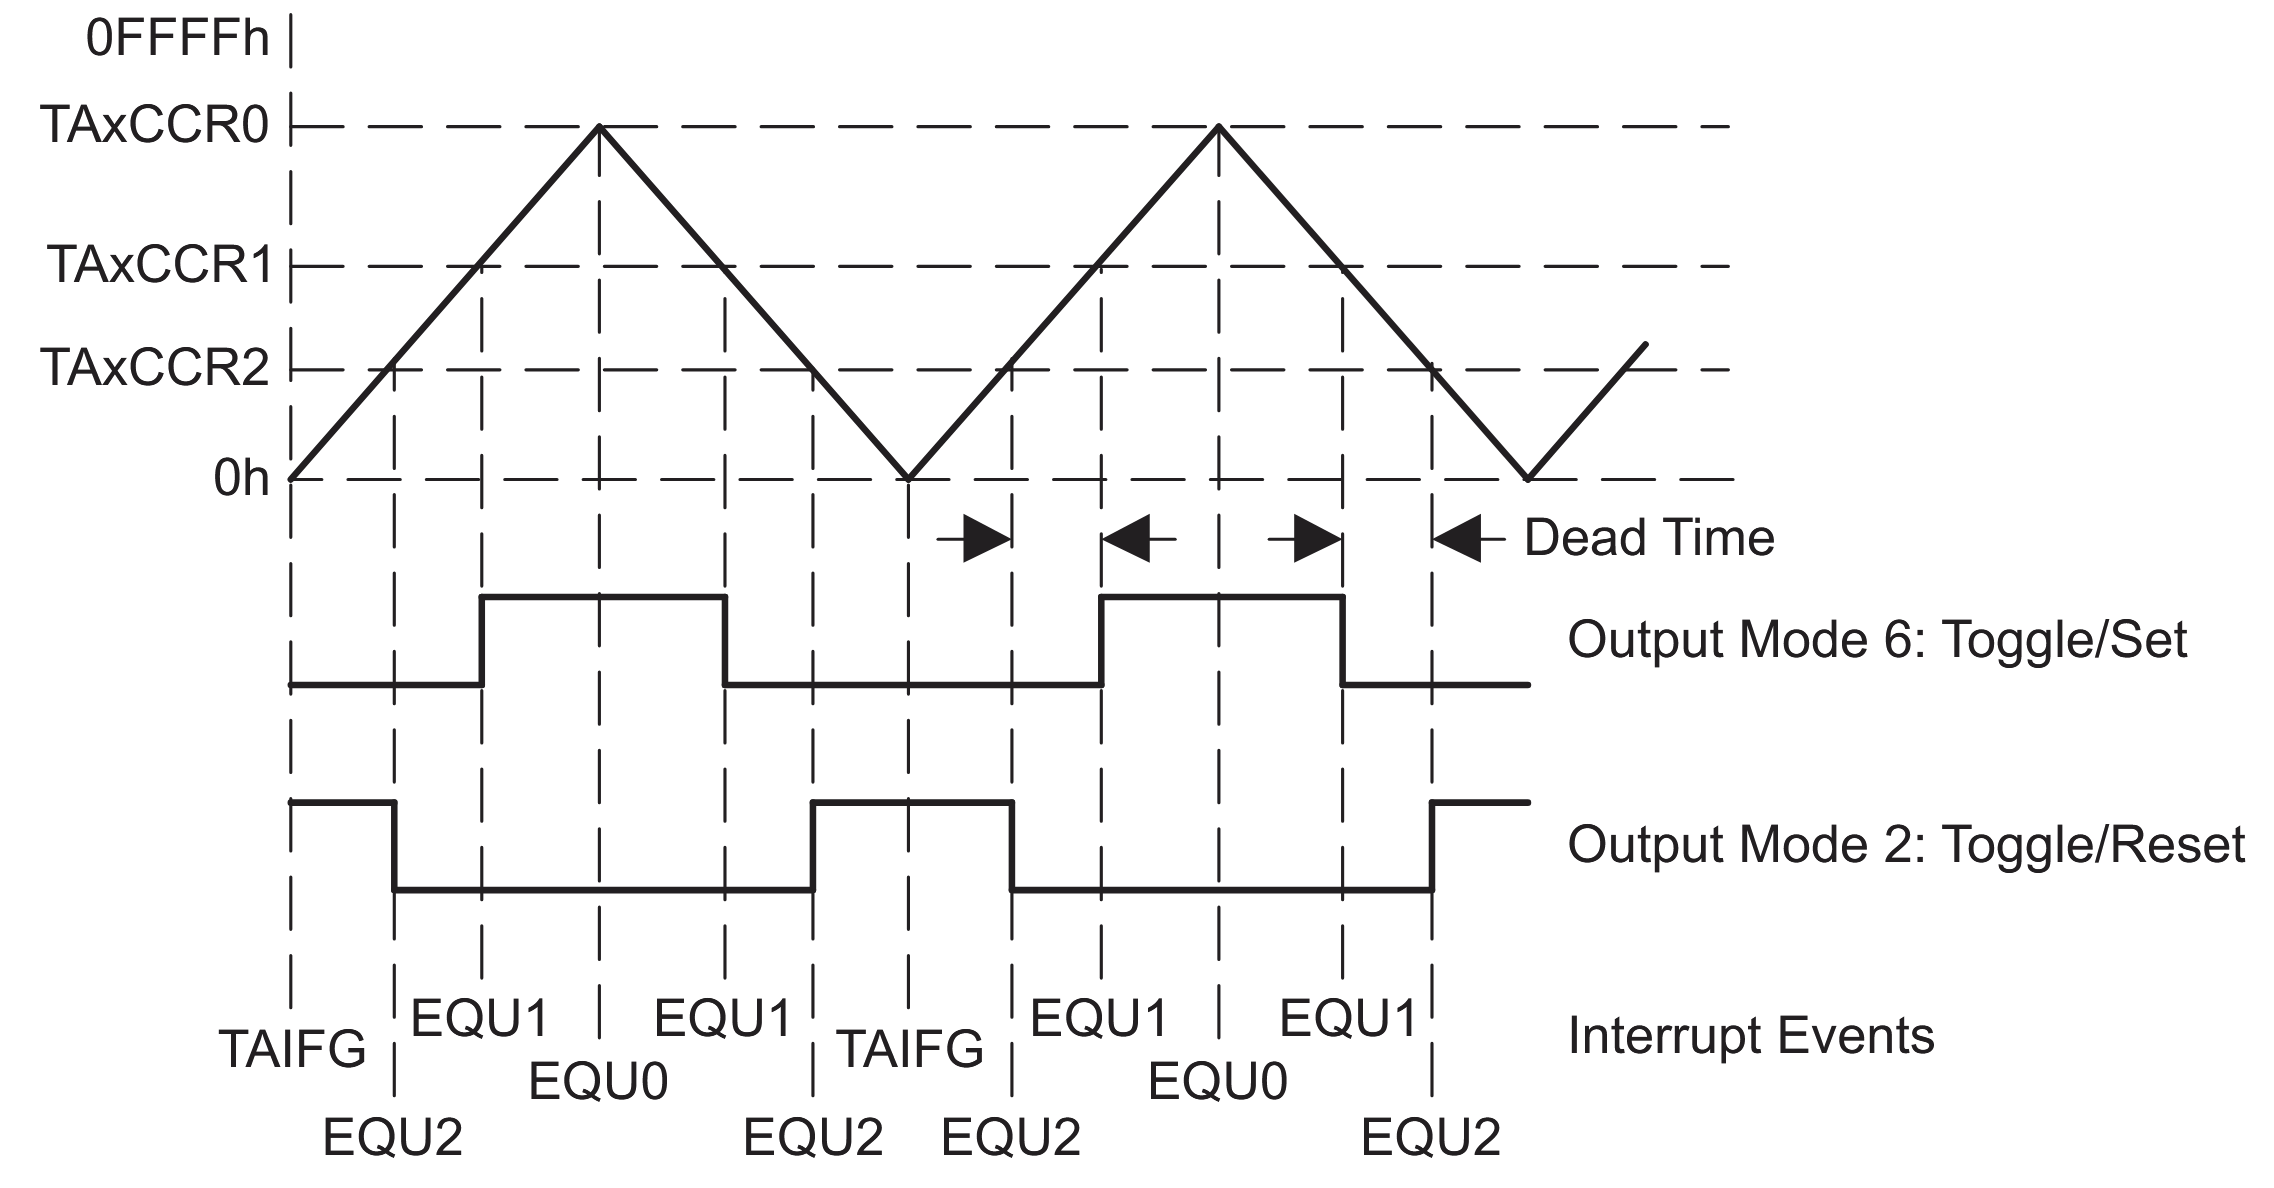
\includegraphics[width=1.0\textwidth]{../Bilder/UpDown_ModeBsp.png}
	\caption{Ausgabeeinheit im Up/Down-Modus\\\Zitat[S. 340, Abb. 11-9]{ti:slau272d}}
	\label{fig:OutputUnit_UpDown_Mode}
\end{figure}

\"Ahnlich wie beim Capture Mode erm\"oglicht ein Interrupt der CPU, auf pr\"azise Zeitpunkte zu reagieren und entsprechende Aktionen auszuf\"uhren. Der Compare Mode ist somit ein vielseitiges Werkzeug zur Erzeugung von Steuersignalen, zur Implementierung von Zeitverz\"ogerungen oder zur Synchronisation interner Operationen mit einer pr\"azisen Zeitbasis. \Zitat[S. 342, Kap. 11.2.4.2 \& S. 364, Kap. 12.2.4.2, S. 352, Kap. 8.8]{ti:slau272d, davies:msp430}

Nachdem die verschiedenen Betriebsarten des Timers betrachtet wurden, ist es wichtig zu verstehen, wie die zugeh\"origen Register konfiguriert werden, um die gew\"unschte Funktionalit\"at zu erzielen.


\subsection{Einstellungen der Capture and Compare Register}
\label{CC_Register}

Die Funktionalit\"at der Capture- und Compare-Einheiten wird ma{\ss}geblich durch die Konfiguration ihrer zugeh\"origen Register bestimmt. Hierzu geh\"oren die Aktivierung und Deaktivierung von Interrupts, die Auswahl des Ausgangsmodus (nur f\"ur Compare) sowie die Festlegung des ausl\"osenden Ereignisses.

F\"ur jedes Capture/Compare-Register kann individuell festgelegt werden, ob ein Interrupt ausgel\"ost werden soll, wenn ein entsprechendes Ereignis eintritt. Dies geschieht \"uber spezifische \NeuerBegriff{Interrupt-Enable-Bits} im jeweiligen Capture/Compare-Control-Register (TAxCCTLn oder TBxCCTLn). Durch das Setzen des CCIE-Bits auf Eins oder Null, kann die Generierung eines Interrupts bei einem Capture- oder Compare-Ereignis aktiviert \bzw deaktiviert werden. \Tabelle{tb_ccc_register} fasst alle weiteren Register des Timers B mit ihren Beschreibungen zusammen.


\begin{table}[h!]
	\small
	\centering
	\begin{tabular}{|c|l|c|c|p{8cm}|}
		\hline
		\textbf{Bit} & \textbf{Field} & \textbf{Type} & \textbf{Reset} & \textbf{Description} \\ \hline
		15-14 & CM & RW & 0h & Capture mode \\ \hline
		13-12 & CCIS & RW & 0h & Capture/compare input select. These bits select the TBxCCRn input signal. \\ \hline
		11 & SCS & RW & 0h & Synchronize capture source. This bit is used to synchronize the capture input signal with the timer clock. \\ \hline
		10-9 & CLLD & RW & 0h & Compare latch load. These bits select the compare latch load event.  \\ \hline
		8 & CAP & RW & 0h & Capture-/Compare mode \\ \hline
		7-5 & OUTMOD & RW & 0h & Output mode. \\ \hline
		4 & CCIE & RW & 0h & Capture/compare interrupt enable. This bit enables the interrupt request of the corresponding CCIFG flag. \\ \hline
		3 & CCI & R & Undef & Capture/compare input. The selected input signal can be read by this bit. \\ \hline
		2 & OUT & RW & 0h & Output. For output mode 0, this bit directly controls the state of the output. \\ \hline
		1 & COV & RW & 0h & Capture overflow. This bit indicates a capture overflow occurred. COV must be reset with software.  \\ \hline
		0 & CCIFG & RW & 0h & Capture/compare interrupt flag \\ \hline
	\end{tabular}
	\caption{Registerbeschreibung – Capture-/Compare Register Timer B\\\Zitat[S. 375, Tab. 12-8]{ti:slau272d}}
	\label{tab:tb_ccc_register}
\end{table}



Wie bereits im Abschnitt \ref{Timer_CompareMode} zum Compare Mode beschrieben, legen die Output Mode Bits (OUTMOD) fest, wie der zugeh\"orige Ausgangspin bei einer \"ubereinstimmung des Z\"ahlerstandes mit dem Compare-Registerwert beeinflusst wird. Die Auswahl des passenden Output Mode ist entscheidend f\"ur die Erzeugung der gew\"unschten Ausgangssignale, wie beispielsweise bei der Pulsweitenmodulation.

Die Auswahl des ausl\"osenden Ereignisses f\"ur eine Capture- oder Compare-Operation wird ebenfalls \"uber Bits im TAxCCTLn- oder TBxCCTLn-Register gesteuert. F\"ur den Capture Mode wird hier beispielsweise mit dem CM-Bit festgelegt, ob die Erfassung bei einer steigenden, fallenden oder beiden Flanken des Eingangssignals erfolgen soll. Im Compare Mode definiert diese Einstellung, unter welchen Bedingungen die Vergleichsoperation als erfolgreich betrachtet wird und die entsprechende Aktion (Interrupt, Ausgangssignal\"anderung) ausgel\"ost wird. Dies kann beispielsweise ein reiner Vergleich oder auch ein Vergleich in Kombination mit dem \"uberlauf des Z\"ahlers im Up Mode sein. \Zitat[S. 351, Kap. 11.3.3 \& S. 375, Kap. 12.3.3, S. 292, Kap. 8.3.2]{ti:slau272d, davies:msp430}

Die sorgf\"altige Konfiguration dieser Einstellungen in den Capture/Compare-Registern ist unerl\"asslich, um den Timer pr\"azise an die Anforderungen der jeweiligen Applikation anzupassen.

Ein weiterer fundamentaler Aspekt der Timer-Konfiguration ist \ua die Wahl der Taktquelle, welche die Zeitbasis f\"ur den Z\"ahler und somit f\"ur alle zeitgesteuerten Operationen des Timers bestimmt. \AI

\newpage
\subsection{Timer Control-Register}
\label{TimerControlRegister}

Die Timer des MSP430FR5729 k\"onnen von verschiedenen internen Taktquellen getaktet werden, die jeweils unterschiedliche Eigenschaften und Anwendungsbereiche aufweisen. Die prim\"aren Taktquellen sind \Fachbegriff[Niederfrequente Taktquelle in Mikrocontroller-Systemen, die typischerweise von einem Quarzoszillator gespeist wird und f\"ur energiesparende Betriebsmodi verwendet wird.]{Auxiliary Clock (ACLK)} und \Fachbegriff[Taktgesteuertes Signal, das typischerweise f\"ur Peripherieger\"ate verwendet wird und sich aus einer frei w\"ahlbaren Taktquelle ableiten l\"asst.]{Sub-Main Clock (SMCLK)}. Auch externe Taktquellen k\"onnen zur Taktung des Timers herangezogen werden wie \zB das TACLK/TBCLK-Register oder der INCLK-Pin. \Zitat[S. 71, Kap. 3.1, S. 163, Kap. 5.8 \& S. 289, Kap. 8.3.1]{ti:slau272d, davies:msp430}

Die Auswahl der Clock-Source f\"ur einen Timer erfolgt \"uber spezifische Bits im TAxCTL oder TBxCTL Timer Control Register. Das TASSEL-/TBSSEL-Bit legt fest, ob der Timer von TAxCLK/TBxCLK, ACLK, SMCLK oder INCLK getaktet wird. Die Wahl der Clock-Source hat einen direkten Einfluss auf die Timer-Frequenz, wobei die Timer-Frequenz nicht gleich der Frequenz der gew\"ahlten Clock-Source entsprechen muss. Durch optionale Prescaler-Werte wie dem ID-Bit und dem TAIDEX-/TBIDEX-Bit kann die Frequenz weiter individualisiert werden. \Zitat[S. 349, Kap. 11.3.1 \& S. 372, Kap. 12.3.1, S. 289, Kap. 8.3.1]{ti:slau272d, davies:msp430}

\begin{table}[h!]
	\small
	\centering
	\begin{tabular}{|c|l|c|c|p{8cm}|}
		\hline
		\textbf{Bit} & \textbf{Field} & \textbf{Type} & \textbf{Reset} & \textbf{Description} \\ \hline
		15 & Reserved & R & 0h & Reserved. Always reads as 0. \\ \hline
		14–13 & TBCLGRP & RW & 0h & \textbf{TBxCLn group:} Synchronously updates multiple Capture/Compare registers as needed. \\ \hline
		12–11 & CNTL & RW & 0h & Counter length \\ \hline
		10 & Reserved & R & 0h & Reserved. Always reads as 0. \\ \hline
		9–8 & TBSSEL & RW & 0h & clock source select \\ \hline
		7–6 & ID & RW & 0h & \textbf{Input divider:} together with TBIDEX divides the input clock \\ \hline
		5–4 & MC & RW & 0h & \textbf{Mode control:} \ref{Timer_CountMode} \\ \hline
		3 & Reserved & R & 0h & Reserved. Always reads as 0. \\ \hline
		2 & TBCLR & RW & 0h & Clears TBR and control logic. \\ \hline
		1 & TBIE & RW & 0h & Timer\_B interrupt enable \\ \hline
		0 & TBIFG & RW & 0h & Timer\_B interrupt flag \\ \hline
	\end{tabular}
	\caption{Registerbeschreibung – Control Register Timer B\\\Zitat[S. 372, Tab. 12-6]{ti:slau272d}}
	\label{tab:tb_c_register}
\end{table}

Die Timer-Frequenz bestimmt wiederum die Zeitbasis des Timers. Eine h\"ohere Timer-Frequenz f\"uhrt zu einer feineren Zeitaufl\"osung, da der Z\"ahler schneller inkrementiert wird. Dies erm\"oglicht pr\"azisere Zeitmessungen und die Erzeugung von Signalen mit h\"oherer Frequenz. Umgekehrt f\"uhrt eine niedrigere Frequenz zu einer gr\"oberen Zeitaufl\"osung, kann aber den Stromverbrauch reduzieren.

Ein weiteres Steuerbits wie das \NeuerBegriff{Mode Control-Bit (MC)} steuert die bereits in Kapitel \ref{Timer_CountMode} erl\"auterten Z\"ahl-Modi und das TAIE-/TBIE-Bit steuert, ob Interrupts Ein- oder Ausgeschaltet sind.

Die Auswahl der Clock-Source, des Prescalers und weiteren Steuerbits ist daher entscheidend, um die gew\"unschte Zeitbasis, Aufl\"osung und Verhalten f\"ur den zu konfigurierenden Timer zu erreichen um die Anforderungen der jeweiligen Anwendung optimal zu erf\"ullen.

\Tabelle{tb_c_register} fasst alle weiteren Register des Timers B mit ihren Beschreibungen zusammen. \AI

\subsection{Zusammenfassung und Einsatzm\"oglichkeiten}
\label{TimerEinsatzmoeglichkeiten}

Die detaillierte Auseinandersetzung mit der Timer-Architektur des MSP430FR5729 hat die Flexibilit\"at und Leistungsf\"ahigkeit dieser Peripheriekomponente verdeutlicht. Die Unterscheidung zwischen Timer des Typs A und B, die verschiedenen Betriebsarten (Count, Capture, Compare) sowie die vielf\"altigen Einstellm\"oglichkeiten der Capture/Compare-Register und die Auswahl der Taktquelle eröffnen ein breites Spektrum an Anwendungsm\"oglichkeiten in eingebetteten Systemen.

Analog zur \"Ubersicht "What Timer Where?" von John H. Davies lassen sich die prim\"aren Einsatzgebiete der Timer des MSP430FR5729 wie folgt zusammenfassen: \Zitat[S. 356, Kap. 8.10]{davies:msp430}

\begin{itemize}
	\item \textbf{Zeitmessung und Zeitbasis:} Unabh\"angig vom Timer-Typ können alle als eine präzise Zeitbasis dienen. Durch die Wahl einer geeigneten Clock-Source und eines passenden Prescalers lassen sich genaue Zeitintervalle festlegen. Dies ist fundamental für das Zeitmanagement innerhalb des Mikrocontrollers und die Synchronisation mit externen als auch Internen Ereignissen. Timer A eignet sich hierbei oft für grundlegende Zeitsteuerungsaufgaben, w\"ahrend die flexiblere Konfigurierbarkeit des Timers vom Typ B wie \zB verschiedene Bit-Längen (\ref{TIMER&ISR}) eine feinere Anpassung an spezifische Zeitmessanforderungen erlaubt.

	\item \textbf{Ereigniserfassung (Capture):} Die Capture-Funktionalit\"at erm\"oglicht die pr\"azise Erfassung des Zeitpunkts externer Ereignisse. Dies ist unerl\"asslich für Anwendungen wie die Messung von Pulsweiten, die Frequenzmessung von Signalen oder die Erfassung der Ankunftszeit von Informationen in Kommunikationsprotokollen. Die M\"oglichkeit, sowohl steigende, fallende Flanken oder auch beide zu erfassen, erweitert den Anwendungsbereich in verschiedenen Szenarien deutlich.

	\item \textbf{Signalerzeugung (Compare/PWM):} Die Compare-Einheiten in Verbindung mit den verschiedenen Ausgangsmodi erlauben die Generierung pr\"aziser Ausgangssignale. Dies ist besonders relevant für die Pulsweitenmodulation, die zur Steuerung von Motoren, zur Dimmung von LEDs oder zur Erzeugung analog wirkender Signale eingesetzt wird. Der Up/Down Mode des Count-Modus in Kombination mit den Compare-Registern des Timer B bietet hierbei besonders flexible M\"oglichkeiten zur Erzeugung verschiedenster PWM-Signale.

	\item \textbf{Interrupt-Steuerung:} Sowohl Capture- als auch Compare-Ereignisse k\"onnen Interrupts ausl\"osen. Dies ermöglicht eine effiziente Reaktion des Mikrocontrollers auf zeitgesteuerte Ereignisse oder externe Signale, ohne die kontinuierliche abfrage des Timer-Status. Die pr\"azise Interrupt-Generierung tr\"agt maßgeblich zur Realisierung reaktiver und effizienter eingebetteter (Echtzeit-) Systeme bei.
\end{itemize}

Zusammenfassend l\"asst sich der grundlegende Aufbau eines Timers, vereinfacht nach dem Vorbild von Abbildung 8.5 und Abbildung 8.16 aus Davies' Buch, wie folgt darstellen:

Ein Timer besteht im Kern aus einem Z\"ahler (\ref{Timer_CountMode}), der durch eine ausgew\"ahlte Clock-Source (\ref{TimerControlRegister}) in definierten Schritten inkrementiert oder dekrementiert wird. Dieser Z\"ahler l\"auft gem\"a{\ss} der gew\"ahlten Betriebsart.

Zus\"atzlich verf\"ugt der Timer \"uber Sieben Capture/Compare-Kan\"ale. Jeder Kanal beinhaltet mindestens ein Capture/Compare-Register und eine zugeh\"orige Steuereinheit.

Im Capture Mode (\ref{Timer_CaptureMode}) wird der aktuelle Wert des Z\"ahlers in das CCRx-Register geschrieben, wenn ein durch die Steuereinheit ausgew\"ahltes Ereignis (\zB Flanke an einem Eingangspin) eintritt.

Im Compare Mode (\ref{Timer_CompareMode}) wird der aktuelle Wert des Z\"ahlers kontinuierlich mit dem Wert im CCRx-Register verglichen. Bei einer \"Ubereinstimmung l\"ost die Steuereinheit eine konfigurierte Aktion aus, wie beispielsweise das Setzen/R\"ucksetzen/Toggeln eines zugeh\"origen Ausgangspins oder die Generierung eines Interrupts, sofern dieser in der Steuereinheit aktiviert wurde.

Die Steuereinheit erm\"oglicht die Konfiguration des jeweiligen Kanals, einschließlich der Auswahl des Capture/Compare-Modus, des ausl\"osenden Ereignisses, des Ausgangsmodus und der Aktivierung/Deaktivierung des Interrupts.

\begin{figure}[h!]
	\centering
	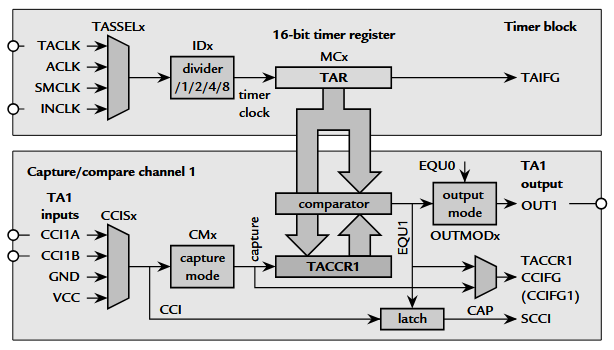
\includegraphics[width=1.0\textwidth]{../Bilder/BlockDiagram_TimerB.png}
	\caption{Timer B Block \& Capture/Compare Channel 1\\\Zitat[S. 355, Kap. 8.16]{davies:msp430}}
	\label{fig:BlockDiagramm_Timer}
\end{figure}

Die Darstellung \Abbildung{BlockDiagramm_Timer} des Timer B als Block Diagram verbildlicht die grundlegenden Komponenten eines Timer-Kanals und deren Zusammenspiel. Die flexiblen Konfigurationsm\"oglichkeiten dieser einzelnen Bl\"ocke erm\"oglichen die Realisierung einer Vielzahl von Zeitsteuerungs- und Signalverarbeitungsaufgaben in eingebetteten Systemen mit dem MSP430FR5729.

\newpage
\section{Enhanced Universal Serial Communication Interface (eUSCI)}
\label{eUSCI}

Das eUSCI ist eine vielschichtige und flexible Serielle Peripheriekomponente des MSP430FR5729. Sie erm\"oglicht die Kommunikation mit externen Ger\"aten und Systemen \"uber eine Vielzahl an Schnittstellen und Protokollen. Auch essentielle Bausteine wie Sensoren, Aktoren und Speichermedien werden \"uber diese Art mit dem System verbunden. Dieses Kapitel beleuchtet die Architektur, verschiedene Betriebsmodi und Konfigurationsm\"oglichkeiten der Bereitgestellten Kommunikationstechnologien.

Der MSP430FR5729 verf\"ugt \"uber zwei Kommunikationskan\"ale welche in den folgenden Kapiteln n\"aher betrachtet werden. 

\subsection{\"Uberblick über die eUSCI-Architektur}
\label{eUSCI_Architektur}

In der Theorie fu{\ss}t jede Form der Seriellen Kommunikation auf einem Taktgeber. Der zentrale Unterschied zwischen den jeweiligen Protokollen liegt darin, zu welchem Zeitpunkt der Taktgeber dem Sender gestattet, das n\"achste Bit auf einen Ausgangskanal zu schreiben, beziehungsweise dem Empf\"anger erm\"oglicht, das kommende Bit zu lesen. Dabei gibt es Synchrone und Asynchrone Ans\"atze, weshalb gleich zwei Kommunikationskan\"ale bereitgestellt werden. \Zitat[S. 494, Kap. 10]{davies:msp430}

Bei dem MSP430FR5729 ist der Kommunikationskanal vom Typ-B f\"ur Synchrone Daten\"ubertragung optimiert, w\"ahrend Kanal A vorrangig f\"ur asynchrone \"Ubertragungsverfahren vorgesehen ist. \Zitat[S. 496, Kap. 10.1.2]{davies:msp430}

Der wesentliche Unterschied zwischen diesen beiden \"Ubertragungsarten besteht darin, ob das Taktsignal ebenfalls mit \"ubertragen wird. Bei der synchronen Kommunikation, wie sie etwa mit den Protokollen SPI oder I$^{2}$C erfolgt, wird dieses Taktsignal explizit mitgef\"uhrt. Im Gegensatz dazu kommt das UART-Protokoll ohne ein separates Taktsignal aus da Sender und Empf\"anger \"uber eine gemeinsame Baudrate synchronisiert sind. \Zitat[S. 494, Kap. 10]{davies:msp430}

\newpage
Entsprechend ist der Univers\"alle Kommunikationskanal vom Typ B (\Abkuerzung{enhanced Universal Serial Communication Interface Type B}{eUSCI\_B}) speziell auf die Anforderungen synchroner Protokolle wie SPI und I$^{2}$C ausgelegt. Das \Abkuerzung{enhanced Universal Serial Communication Interface Type A}{eUSCI\_A}-Modul hingegen unterst\"utzt prim\"ar die UART-Kommunikation, kann jedoch dar\"uber hinaus auch eine asynchrone Variante des SPI-Protokolls abbilden. \Zitat[S. 496, Kap. 10.1.2]{davies:msp430}

\begin{table}[h!]
	\small
	\centering
	\begin{tabular}{|l|c|c|}
		\hline
		\textbf{Funktion} & \textbf{eUSCI\_A} & \textbf{eUSCI\_B} \\\hline
		UART (asynchron) & \checkmark & -- \\\hline
		SPI (synchron) & \checkmark (Master/Slave) & \checkmark (Master/Slave) \\\hline
		SPI (asynchron, nur TX) & \checkmark & -- \\\hline
		I\textsuperscript{2}C (synchron) & -- & \checkmark (Master/Slave) \\\hline
		LIN-kompatibel & \checkmark & -- \\\hline
		Automatische Baudratenerkennung (UART) & \checkmark & -- \\\hline
		Adress- und Broadcast-Modus (I\textsuperscript{2}C) & -- & \checkmark \\\hline
		Multimaster-Unterstützung (I\textsuperscript{2}C) & -- & \checkmark \\\hline
	\end{tabular}
	\caption{Funktionsvergleich der eUSCI-Module des MSP430FR5729\\\Zitat[Kap. 18, 19, 20, S. 493, Kap. 10]{ti:slau272d, davies:msp430}}
	\label{tab:eusci-vergleich}
\end{table}

\Tabelle{eusci-vergleich} fasst nochmals alle Eigenschaften beider Kan\"ale zusammen und stellt sie gegen\"uber. Wobei Tiefgreifendere, Protokoll-Spezifische Funktionen in den entsprechenden Unterkapiteln n\"aher betrachtet werden.

\subsection{eUSCI\_A Modul: UART-Modus (Asynchrone Kommunikation)}
\label{eUSCI_UART}

\subsection{eUSCI\_A und eUSCI\_B Module: SPI-Modus (Synchrone Kommunikation)}
\label{eUSCI_SPI}

\subsection{eUSCI\_B Modul: I$^{2}$C-Modus (Inter-Integrated Circuit)}
\label{eUSCI_I2C}

\subsection{Allgemeine eUSCI-Konfiguration und GPIO-Anbindung}
\label{eUSCI_Konfiguration}

\subsection{Zusammenfassung und Anwendungsbeispiele der eUSCI-Protokolle}
\label{eUSCI_Zusammenfassung}